\documentclass[aspectratio=169]{beamer}

\usepackage[utf8]{inputenc}
\usepackage[T1]{fontenc}
\usepackage[spanish]{babel}
\usepackage{booktabs}
\usepackage{array}
\usepackage{xcolor}
\usepackage{graphicx}

\usetheme{Madrid}
\usecolortheme{default}

\setbeamertemplate{navigation symbols}{}
\setbeamertemplate{footline}[frame number]

\definecolor{okgreen}{RGB}{34,139,34}
\definecolor{warnorange}{RGB}{204,102,0}
\definecolor{badred}{RGB}{178,34,34}

\title[Detección de Enfermedades en Cultivos]{Sistema Inteligente para la Detección de\\Enfermedades en Cultivos mediante CNN}
\subtitle{Resultados finales del proyecto — Organización por roles del equipo}
\author{Grupo 2}
\date{16 de julio de 2026}

\begin{document}

% ---------------------------------------------------------
\begin{frame}
  \titlepage
\end{frame}

% ---------------------------------------------------------
\begin{frame}{Agenda}
  \tableofcontents
\end{frame}

% ===========================================================
\section{Contexto y Dataset}

\begin{frame}{Contexto del proyecto}
  \begin{block}{El problema}
    Una cooperativa agrícola necesita una aplicación que permita diagnosticar enfermedades en hojas de cultivos a partir de fotografías tomadas con un celular.
  \end{block}
  \begin{itemize}
    \item El sistema debe exponer sus predicciones a través de una \textbf{API} y una \textbf{interfaz web} simple.
    \item Objetivo: analizar el dataset, entrenar y comparar dos modelos de Deep Learning, y desplegar el mejor modelo como un servicio consumible desde la web.
  \end{itemize}
\end{frame}

\begin{frame}{El dataset}
  \centering
  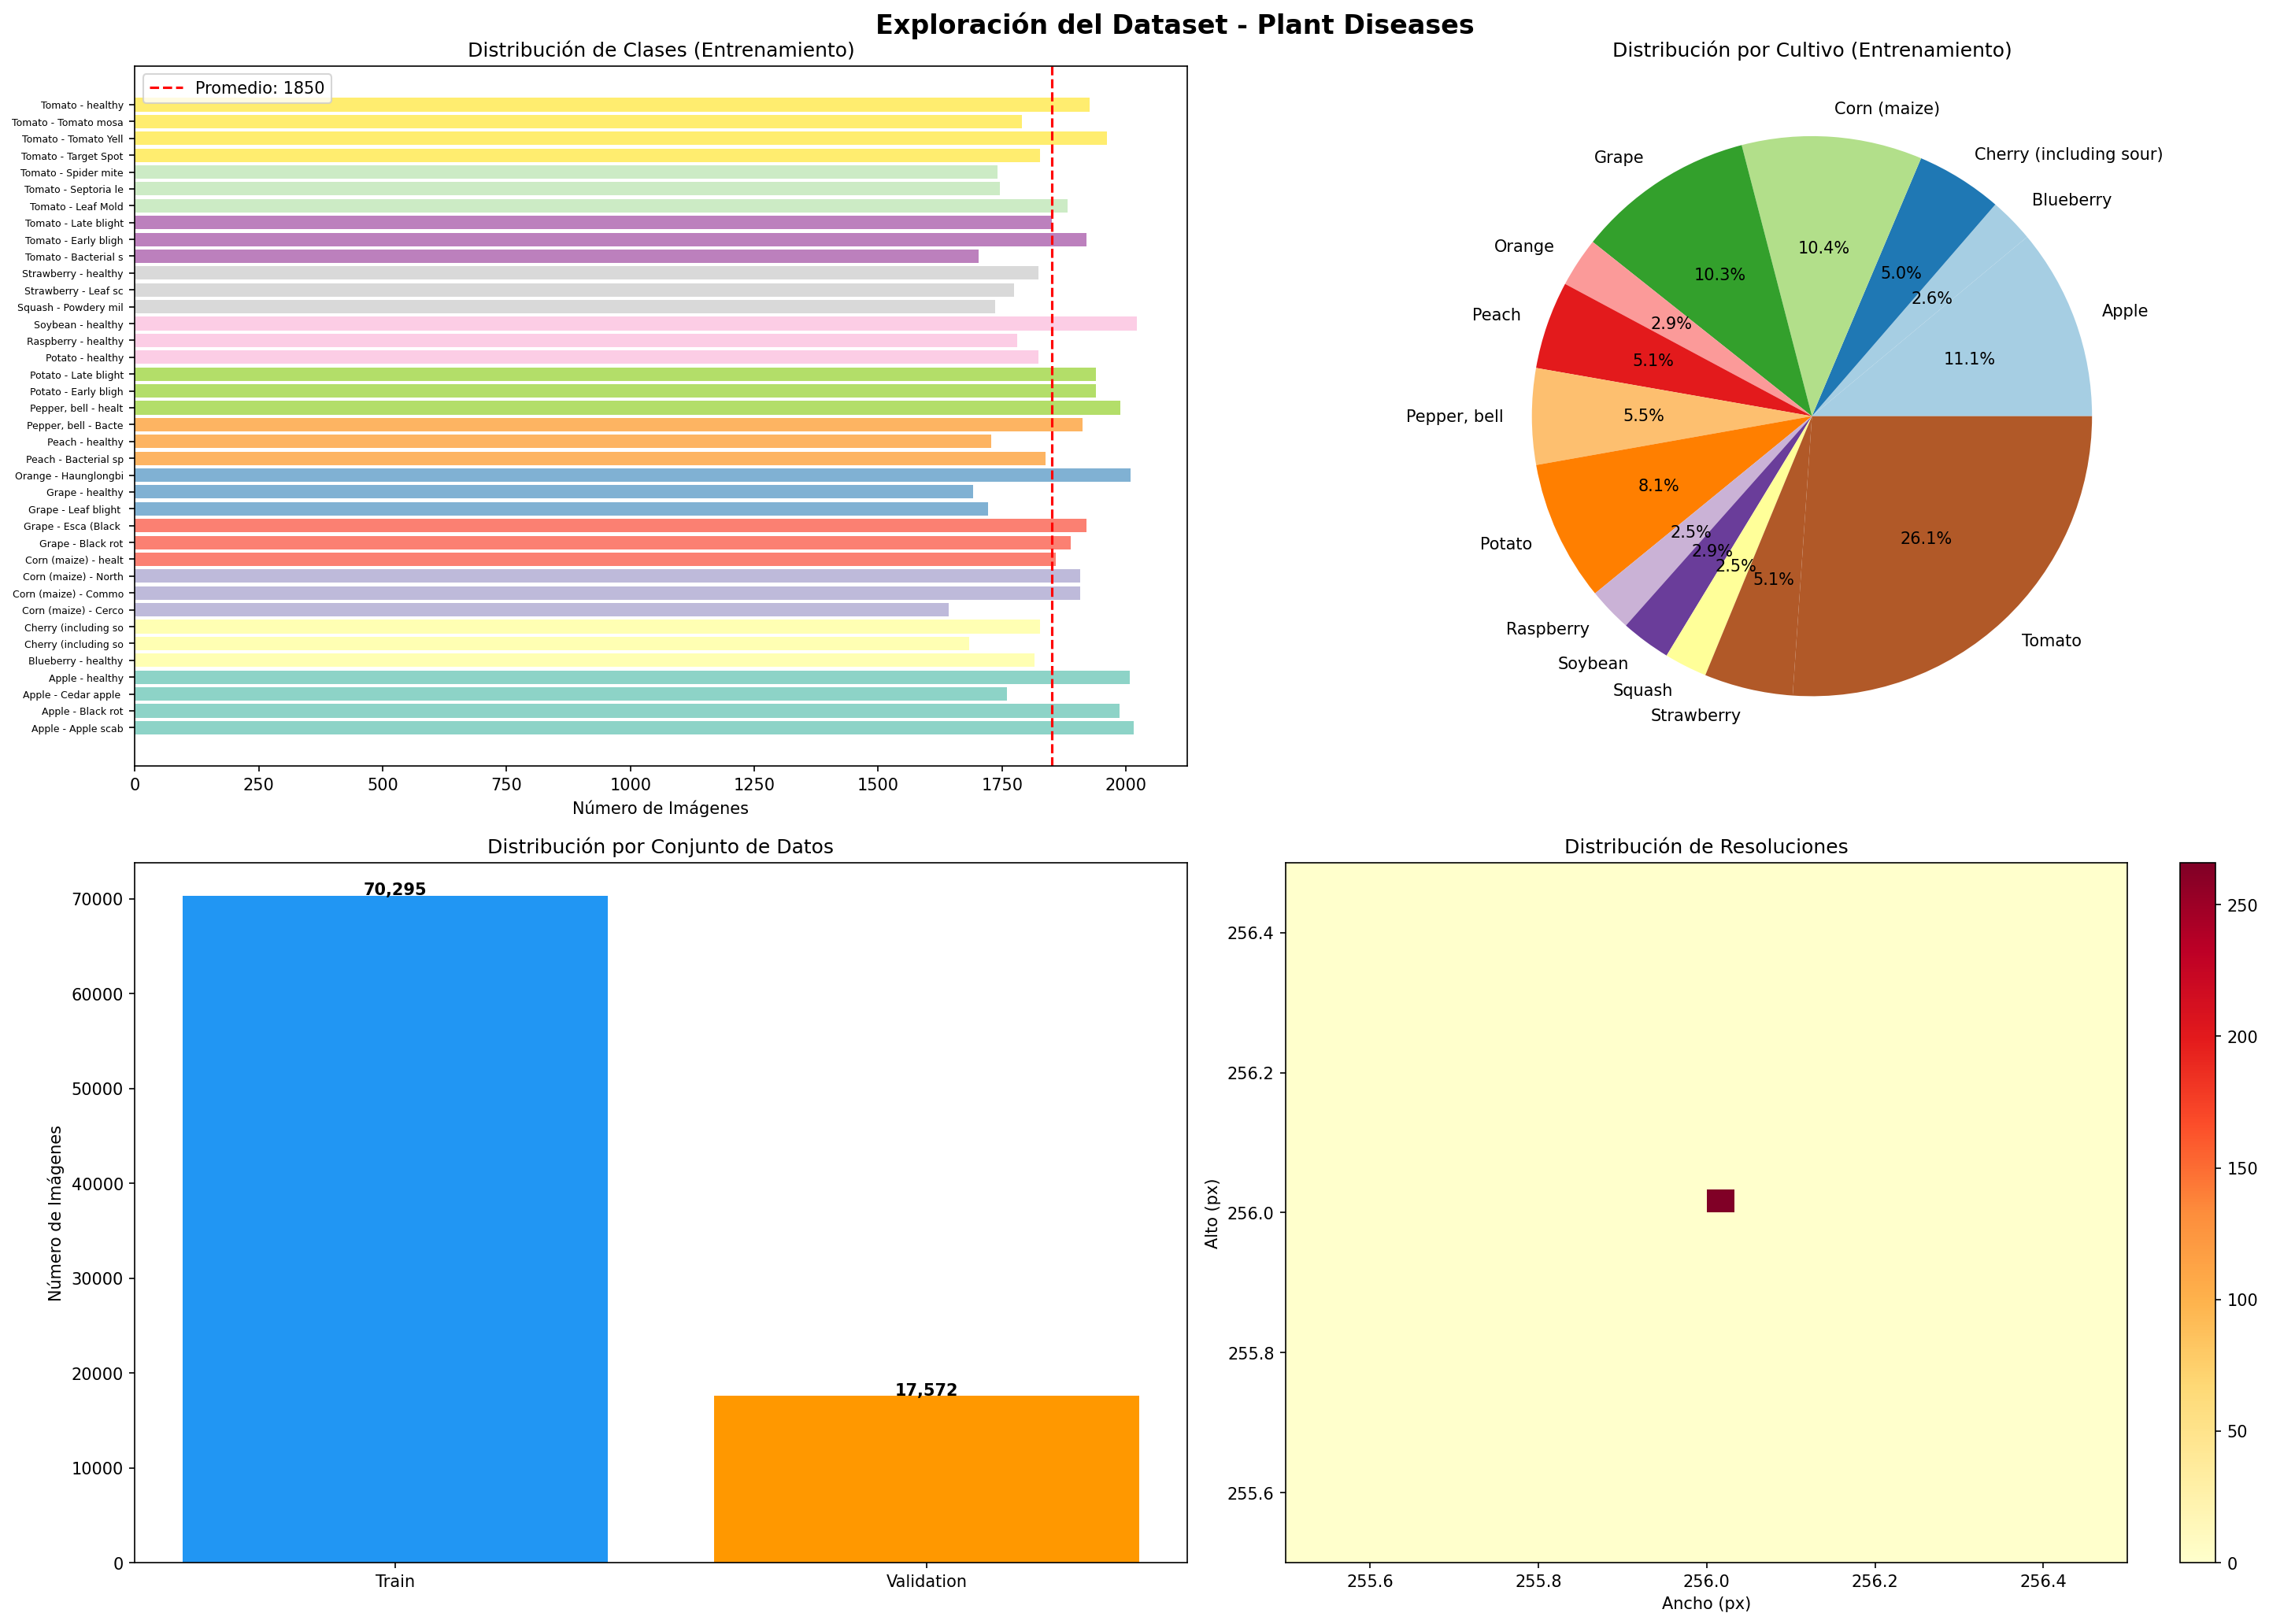
\includegraphics[width=0.6\textwidth]{images/eda_analysis.png}
  \vspace{0.2cm}
  \footnotesize
  \begin{itemize}
    \item \textbf{Fuente}: ``New Plant Diseases Dataset'' (Kaggle), $\sim$3\,GB, imágenes ya normalizadas a 256$\times$256\,px.
    \item \textbf{38 clases} = 14 cultivos $\times$ sus enfermedades (o estado sano). Ej.: \texttt{Tomato\_\_\_Early\_blight}, \texttt{Apple\_\_\_healthy}.
    \item \textbf{87{,}867 imágenes} en total: 70{,}295 de entrenamiento y 17{,}572 de validación (split 80/20).
    \item Dataset razonablemente balanceado entre clases (1{,}650–2{,}020 imágenes c/u), aunque Tomate concentra 26\% del total por tener 10 subtipos de enfermedad distintos.
  \end{itemize}
\end{frame}

\begin{frame}{Composición del equipo}
  \begin{itemize}
    \item El proyecto original está pensado para 7 roles especializados (Líder, Ingeniero de Datos, Especialista en Deep Learning, Investigador, Backend, DevOps/QA, Frontend).
    \item Con un equipo de \textbf{3 integrantes}, cada persona asume varios roles combinados.
    \item El trabajo se organizó en \textbf{3 perfiles}, cada uno responsable de un tramo completo del pipeline: datos/modelos, backend/despliegue, y frontend/QA.
  \end{itemize}
\end{frame}

% ===========================================================
\section{Rol 1 — Data Scientist / Deep Learning Lead}

\begin{frame}{Rol 1 — Responsabilidades}
  \begin{block}{Equivalente a: Líder + Ingeniero de Datos + Especialista en Deep Learning + Investigador}
  \end{block}
  \begin{itemize}
    \item Explora el dataset (clases, balance, resolución, cultivos).
    \item Realiza el preprocesamiento y Data Augmentation.
    \item Diseña y entrena la CNN propia.
    \item Aplica y compara Transfer Learning (ResNet50).
    \item Calcula métricas de evaluación y genera las curvas y matriz de confusión.
  \end{itemize}
\end{frame}

\begin{frame}{Preprocesamiento y balance de clases}
  \centering
  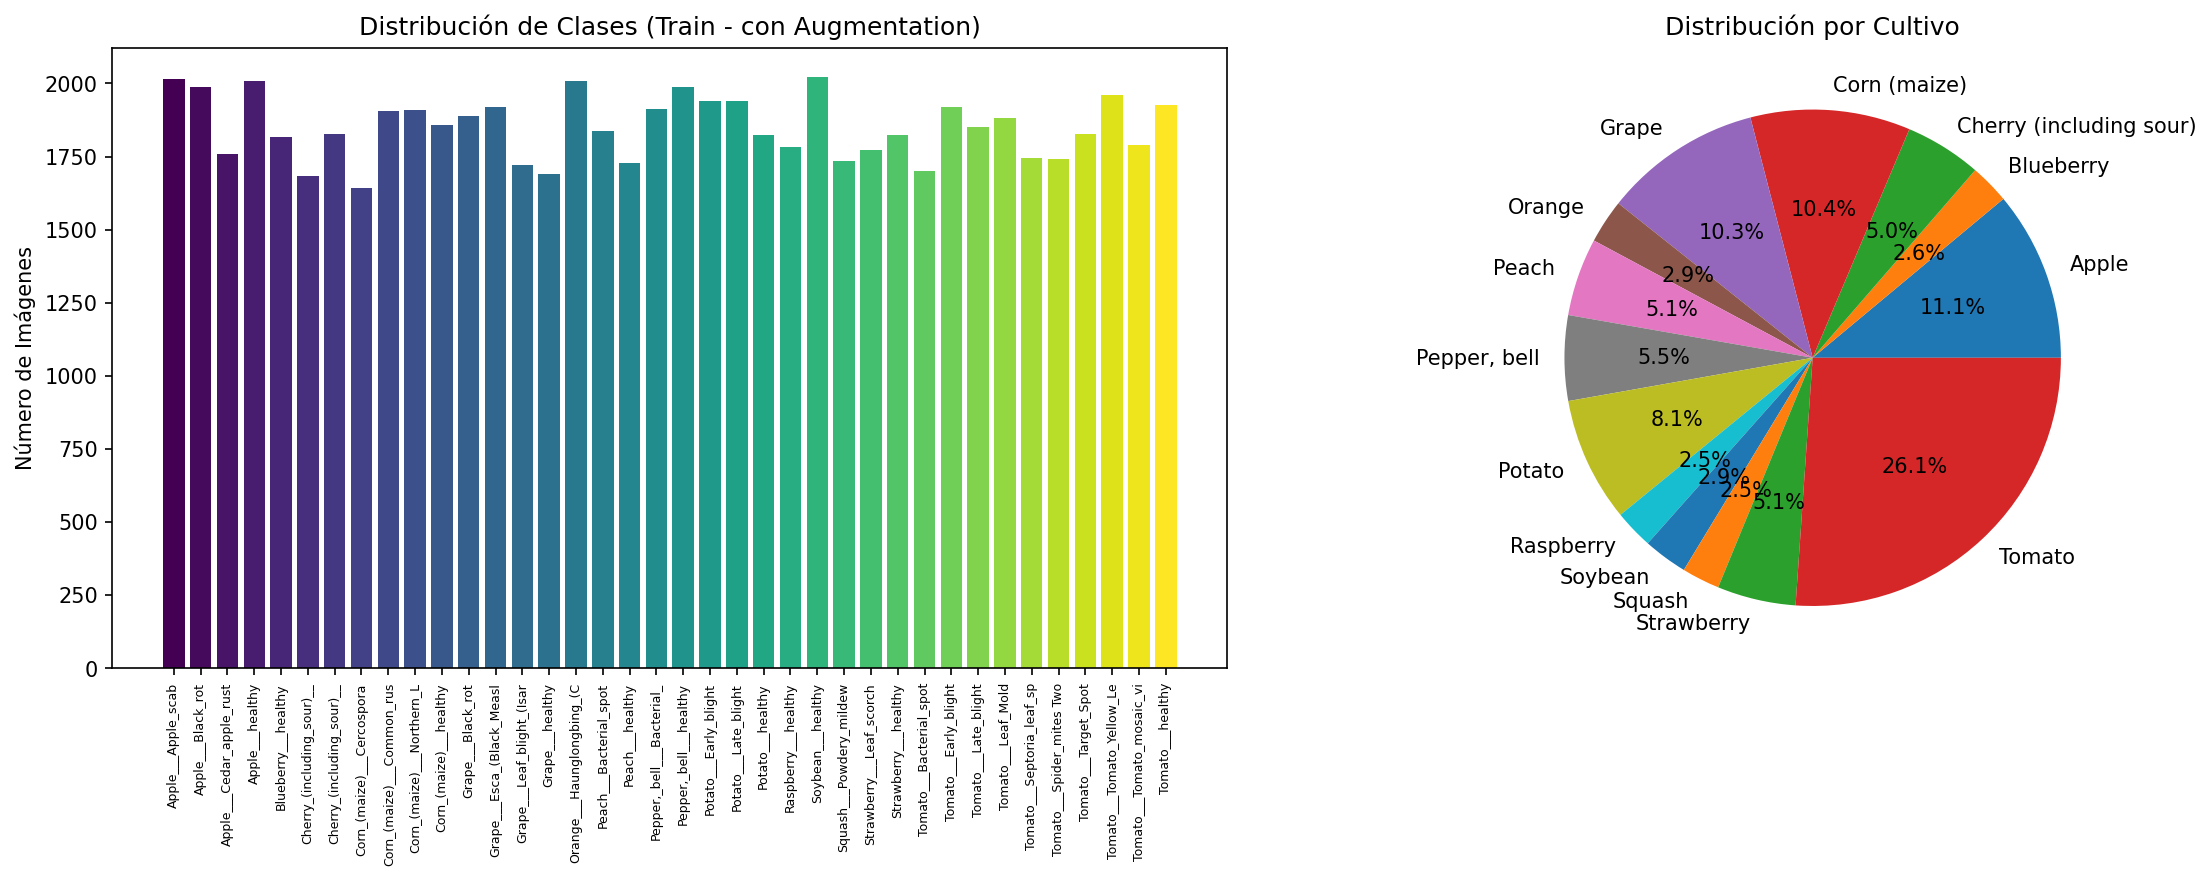
\includegraphics[width=0.55\textwidth]{images/class_distribution_preprocessed.png}
  \vspace{0.2cm}
  \footnotesize
  \begin{itemize}
    \item Tras el Data Augmentation la distribución por clase queda aún más pareja (todas entre 1{,}650 y 2{,}020 imágenes).
    \item Las proporciones por cultivo se mantienen; el objetivo era asegurar suficientes ejemplos por cada clase individual, no cambiar el balance entre cultivos.
  \end{itemize}
\end{frame}

\begin{frame}{Ejemplo de Data Augmentation}
  \centering
  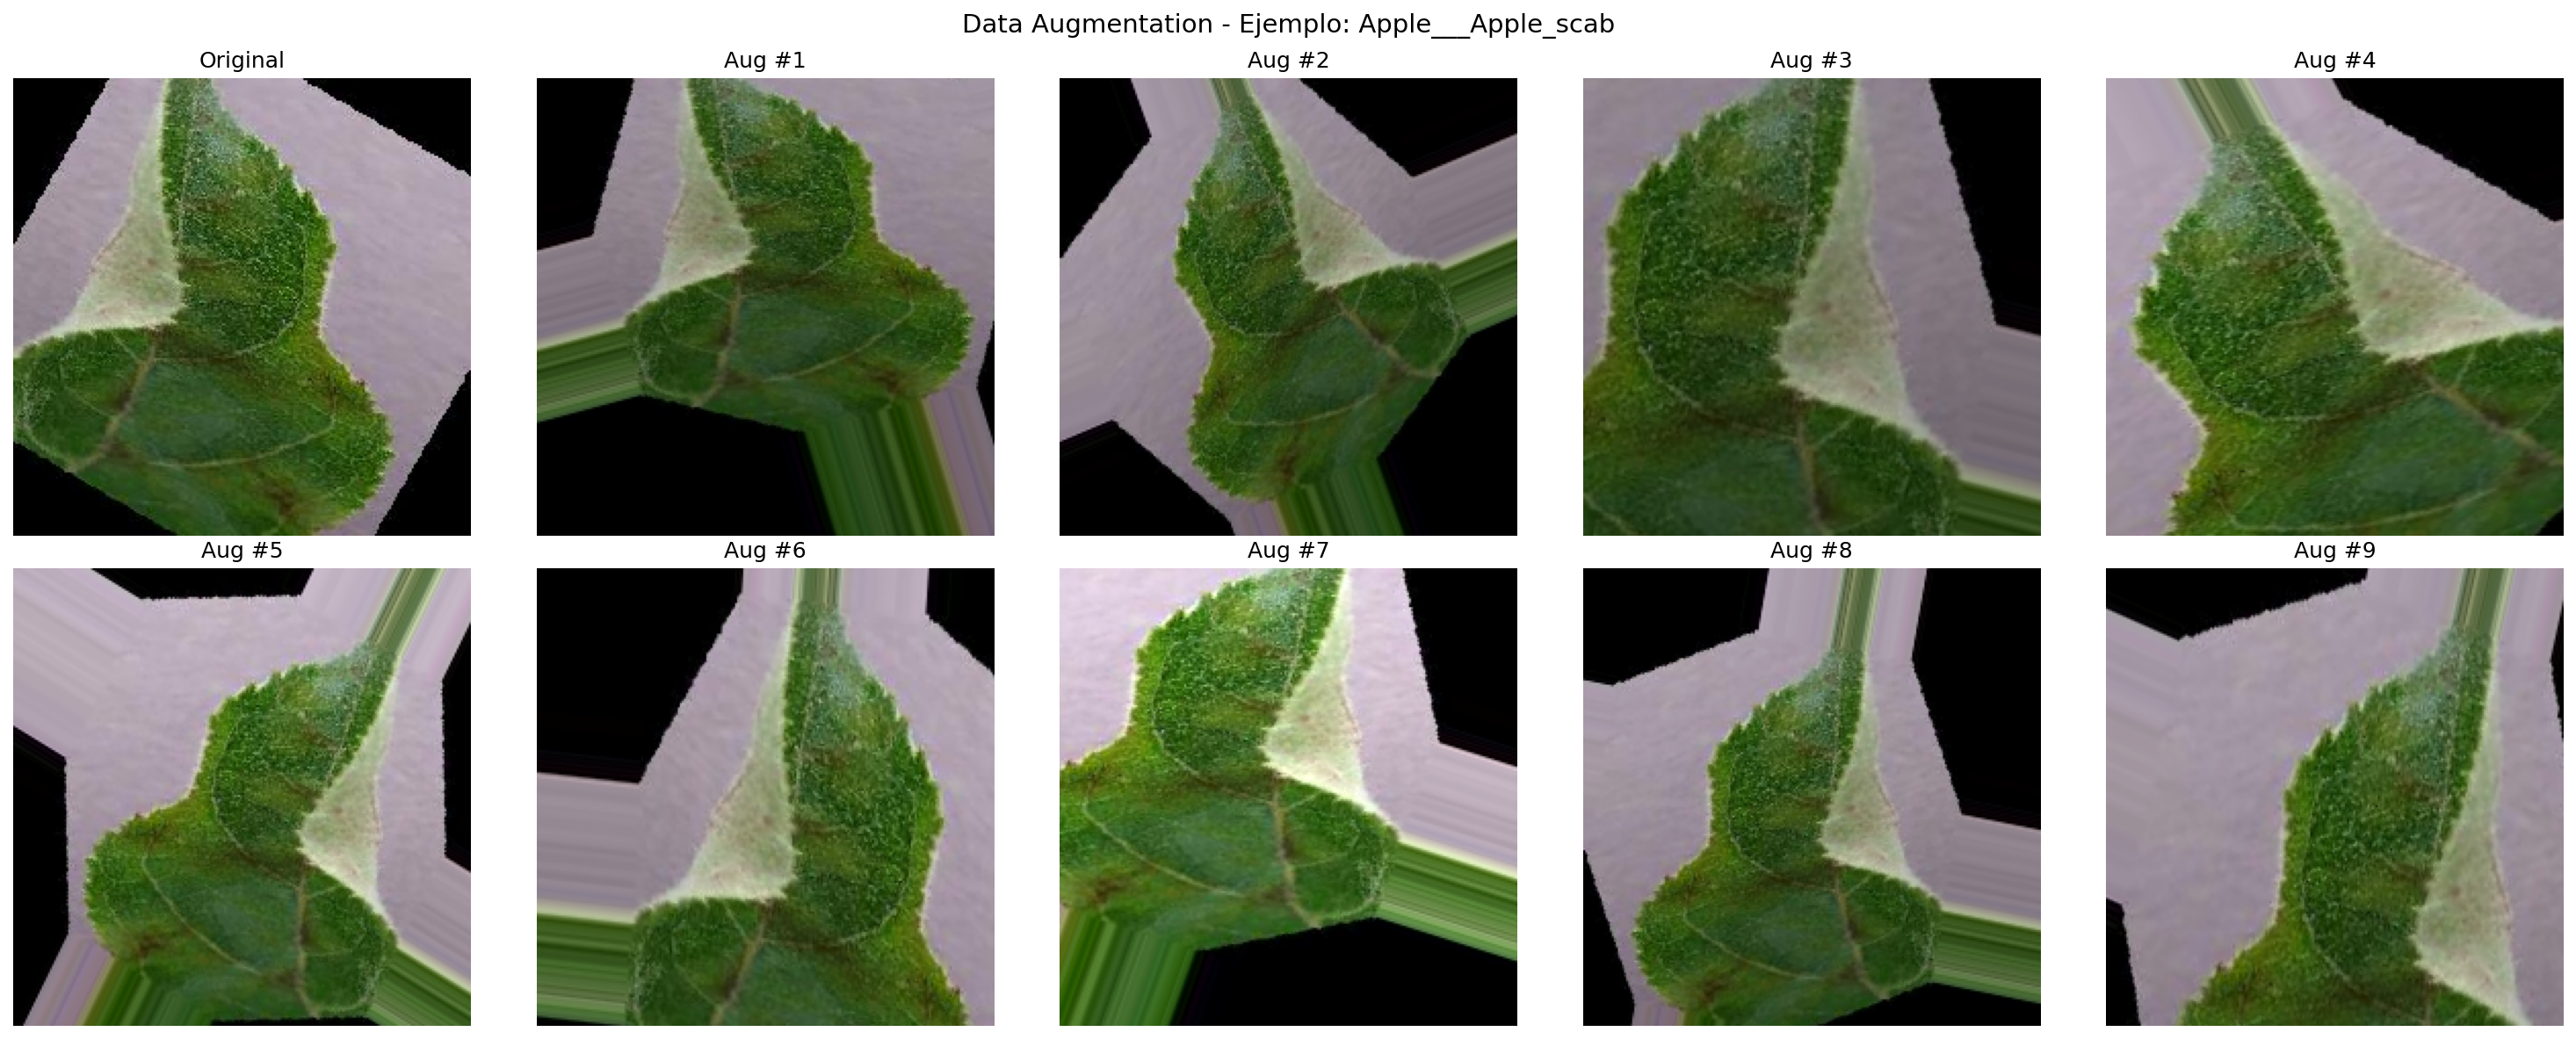
\includegraphics[width=0.68\textwidth]{images/data_augmentation_example.png}
  \vspace{0.2cm}
  \footnotesize
  \begin{itemize}
    \item Misma hoja transformada 9 veces: rotaciones, recortes/zoom y cambios de color/brillo.
    \item El objetivo es que el modelo no memorice el ángulo o la iluminación exacta de cada foto, sino la forma y textura de la lesión.
  \end{itemize}
\end{frame}

\begin{frame}{CNN propia: resultado}
  \begin{block}{Arquitectura}
    4 bloques convolucionales (32 $\to$ 64 $\to$ 128 $\to$ 256 filtros) con BatchNorm y Dropout, sin usar ningún modelo preentrenado.
  \end{block}
  \centering
  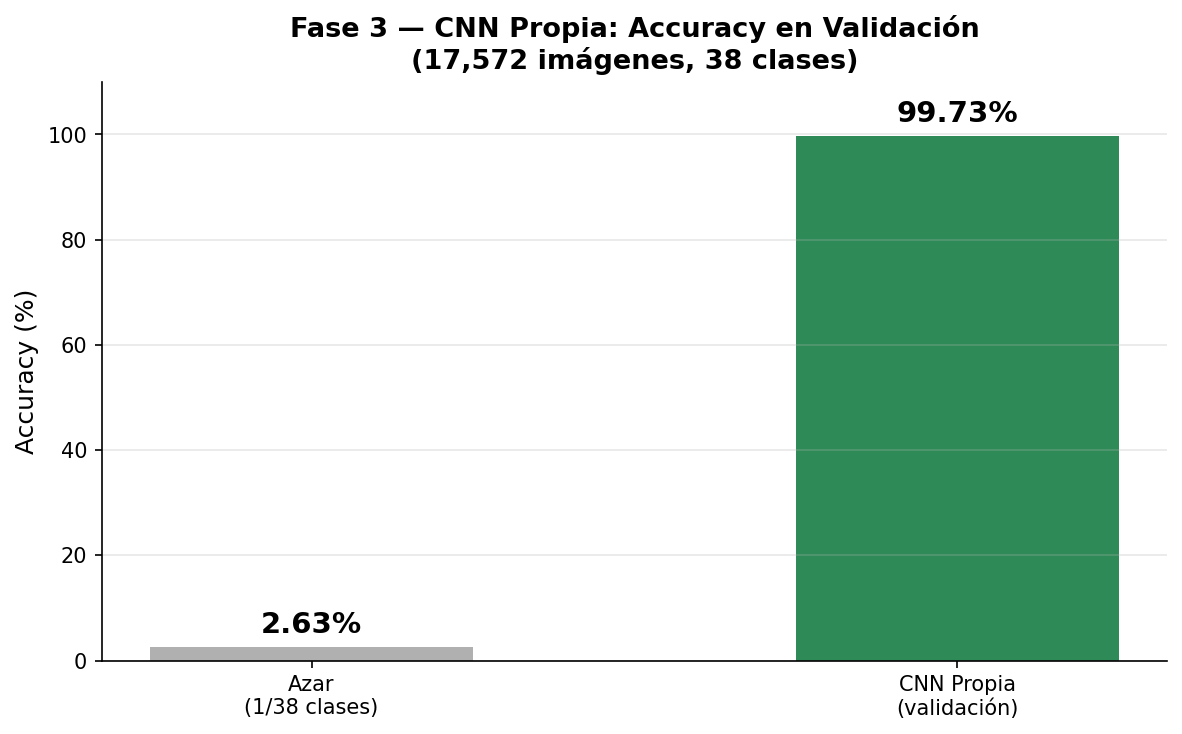
\includegraphics[width=0.42\textwidth]{images/cnn_custom_result.png}
  \vspace{0.15cm}
  \footnotesize
  \begin{itemize}
    \item 99.73\% de accuracy en validación, muy por encima del azar (2.63\%, 1 de 38 clases).
    \item Entrenada en Kaggle mediante ``Save Version'' (ejecución en segundo plano, sin depender de mantener el navegador abierto).
  \end{itemize}
\end{frame}

\begin{frame}{CNN propia: curvas de entrenamiento}
  \centering
  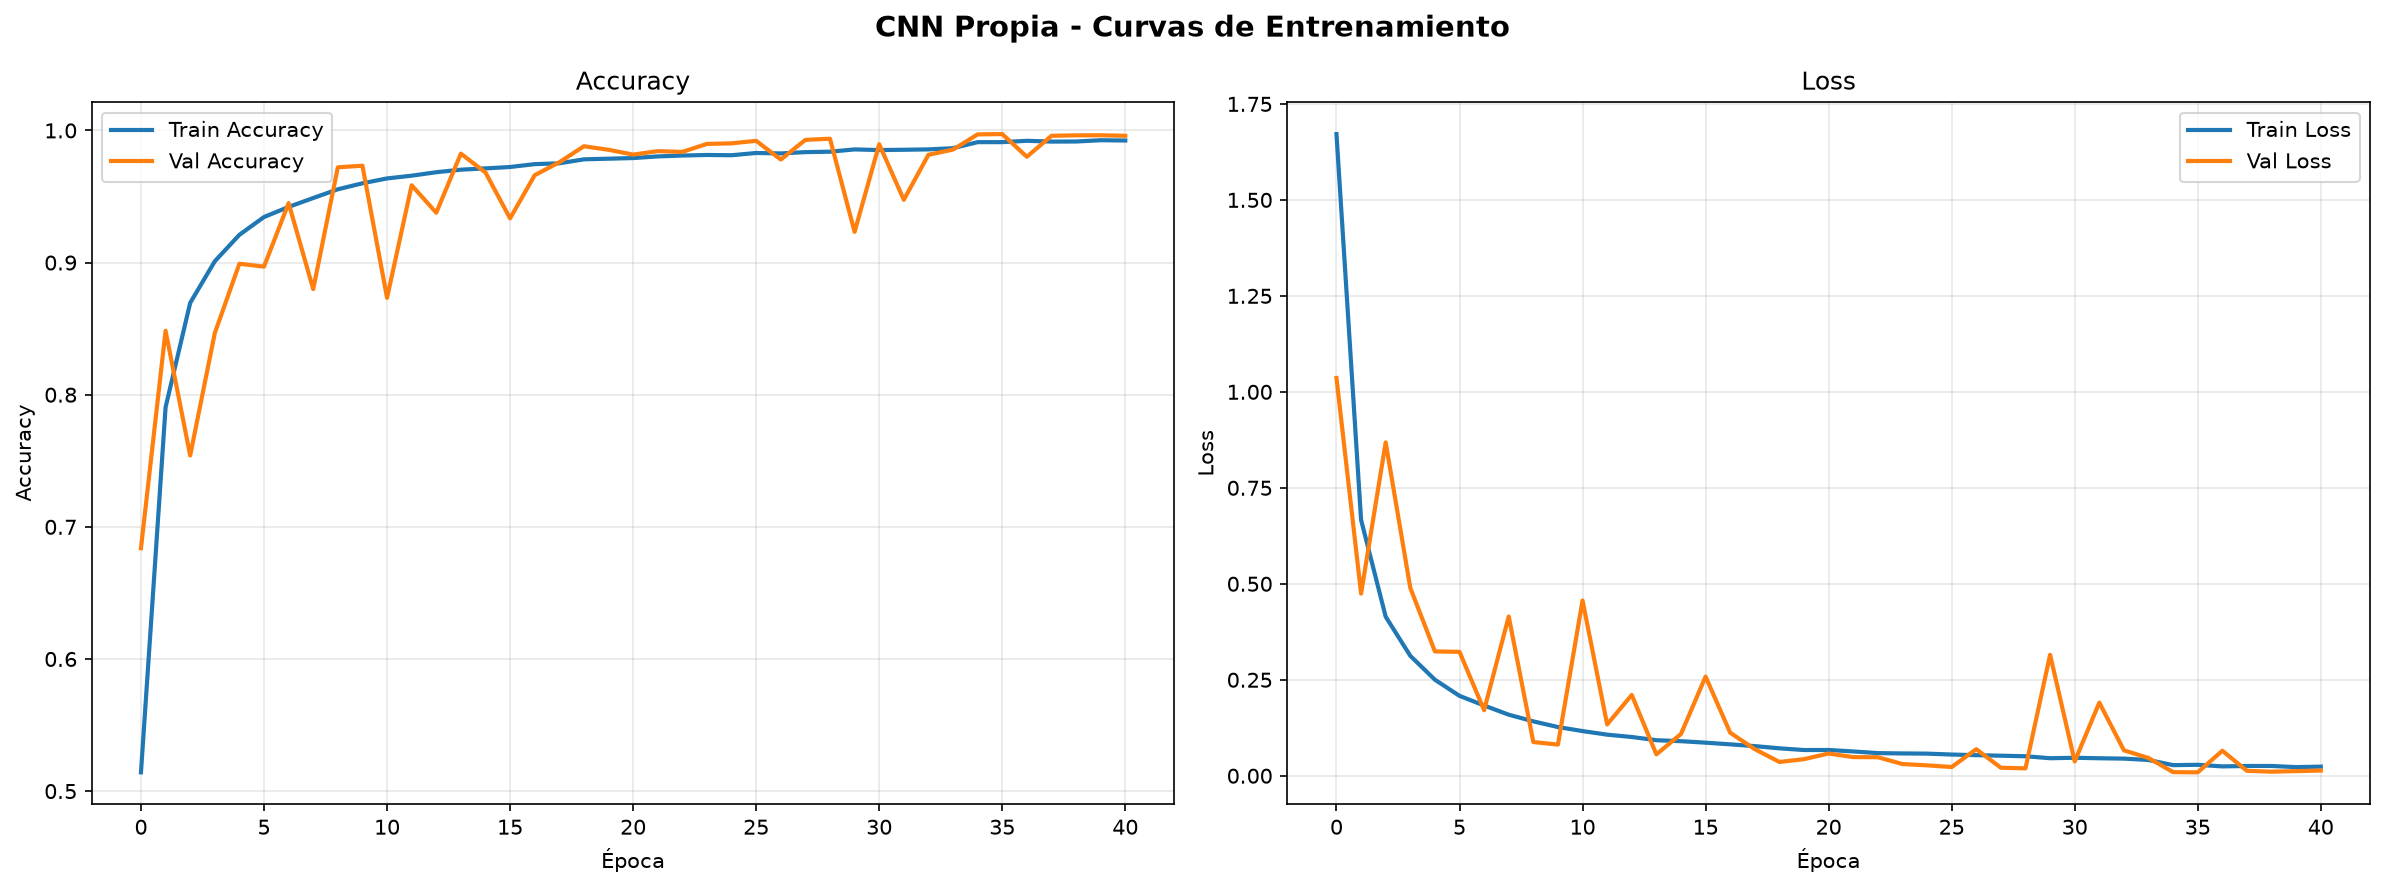
\includegraphics[width=0.56\textwidth]{images/cnn_custom_training.png}
  \vspace{0.1cm}
  \footnotesize 41 épocas: el accuracy de validación converge rápido (supera 90\% desde la época 5) y se estabiliza cerca del 99\%; mejor checkpoint en la época 36 (99.73\%), sin señales de sobreajuste en el loss.
\end{frame}

\begin{frame}{Transfer Learning — ResNet50}
  \begin{itemize}
    \item Un primer intento de entrenamiento local se interrumpió antes de completarse; se repitió con el mismo enfoque de ``Save Version'' en Kaggle que funcionó para la CNN propia.
    \item Segundo intento: \textbf{30 épocas completas en $\sim$8.7 horas}, sin interrupciones.
    \item \textbf{Resultado: 76.9\% de accuracy en validación.}
  \end{itemize}
  \centering
  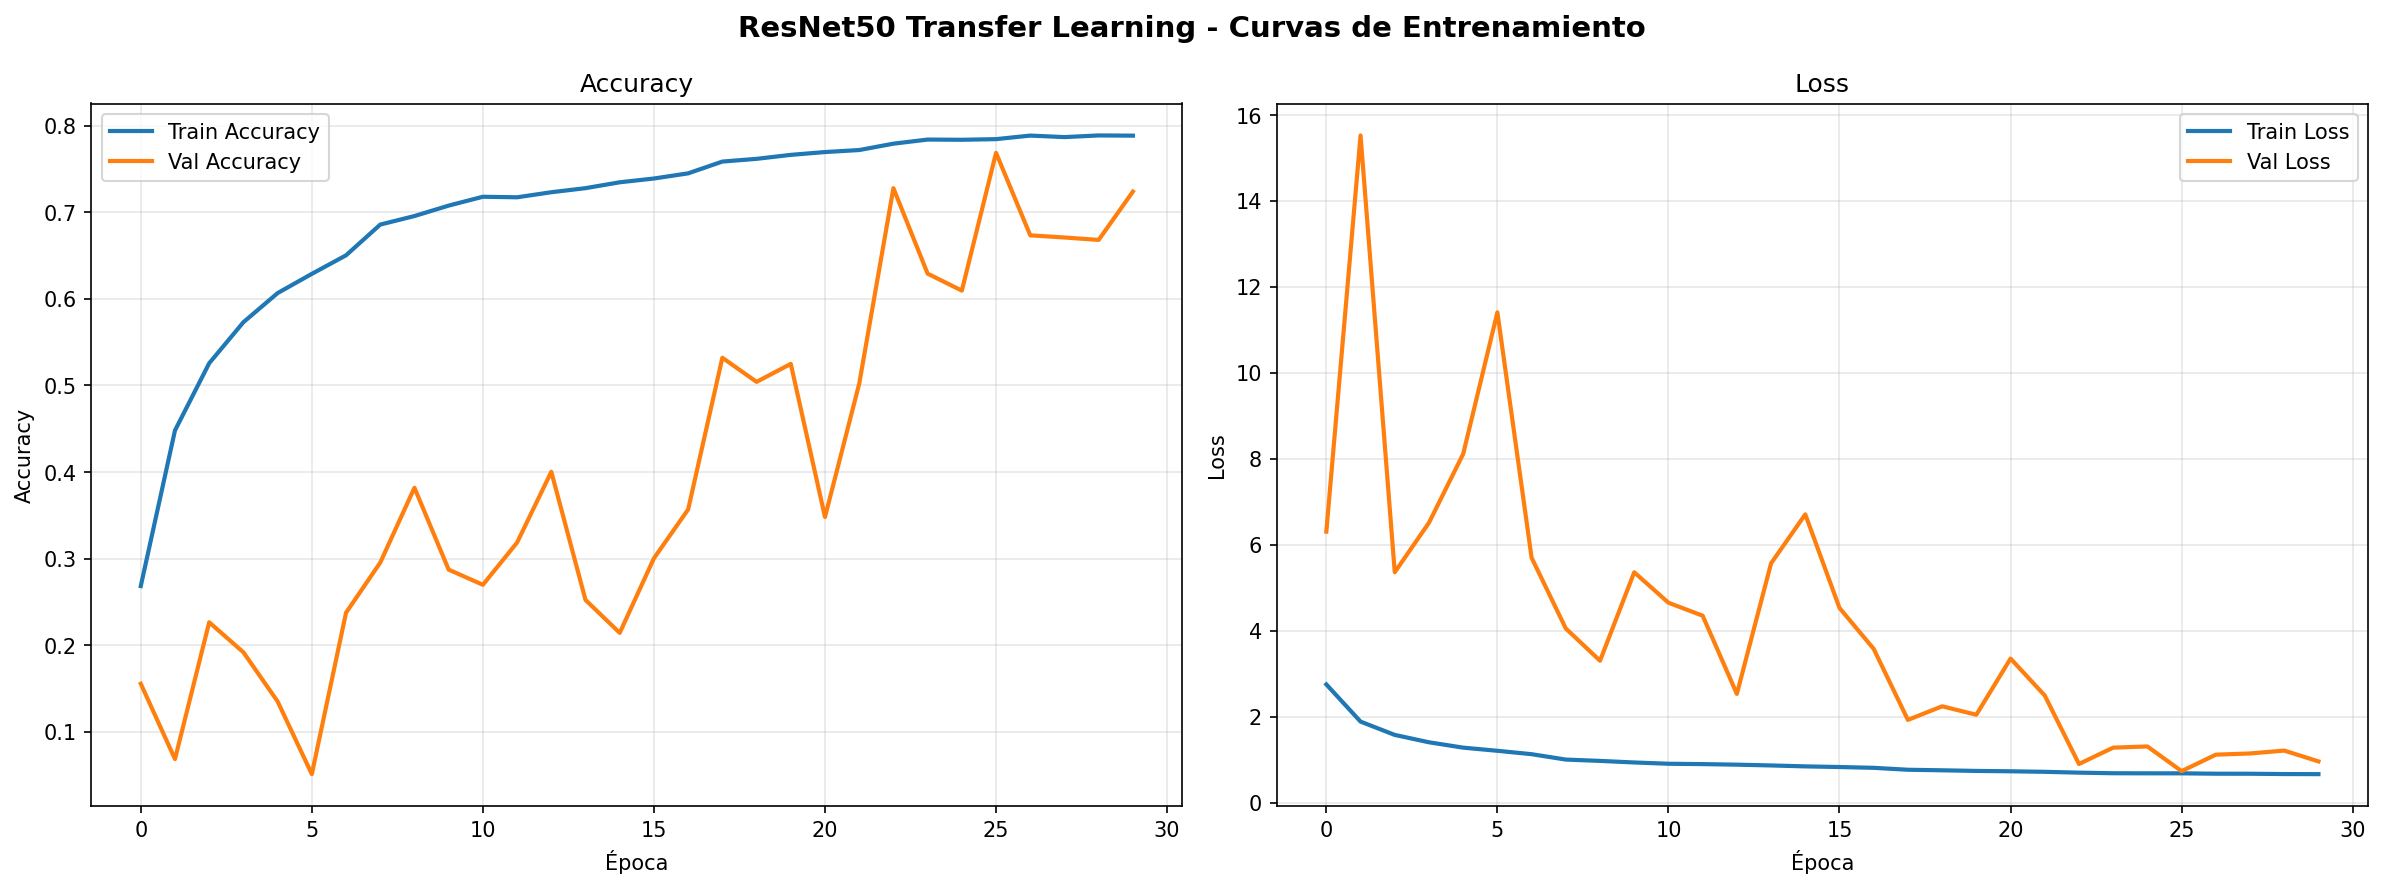
\includegraphics[width=0.56\textwidth]{images/resnet50_training.png}
  \vspace{0.1cm}
  \footnotesize El accuracy de entrenamiento sube establemente hasta $\sim$78\%; el de validación es mucho más ruidoso, por lo que se guarda el mejor checkpoint (época 26) en vez de la última época.
\end{frame}

\begin{frame}{Evaluación comparativa: CNN propia vs. ResNet50}
  \centering
  \begin{tabular}{lcc}
    \toprule
    \textbf{Métrica} & \textbf{CNN propia} & \textbf{ResNet50} \\
    \midrule
    Accuracy & 99.7\% & 76.9\% \\
    Precisión & 99.7\% & 80.7\% \\
    Recall & 99.7\% & 76.9\% \\
    F1-score & 99.7\% & 75.8\% \\
    \bottomrule
  \end{tabular}
  \vspace{0.3cm}
  \centering
  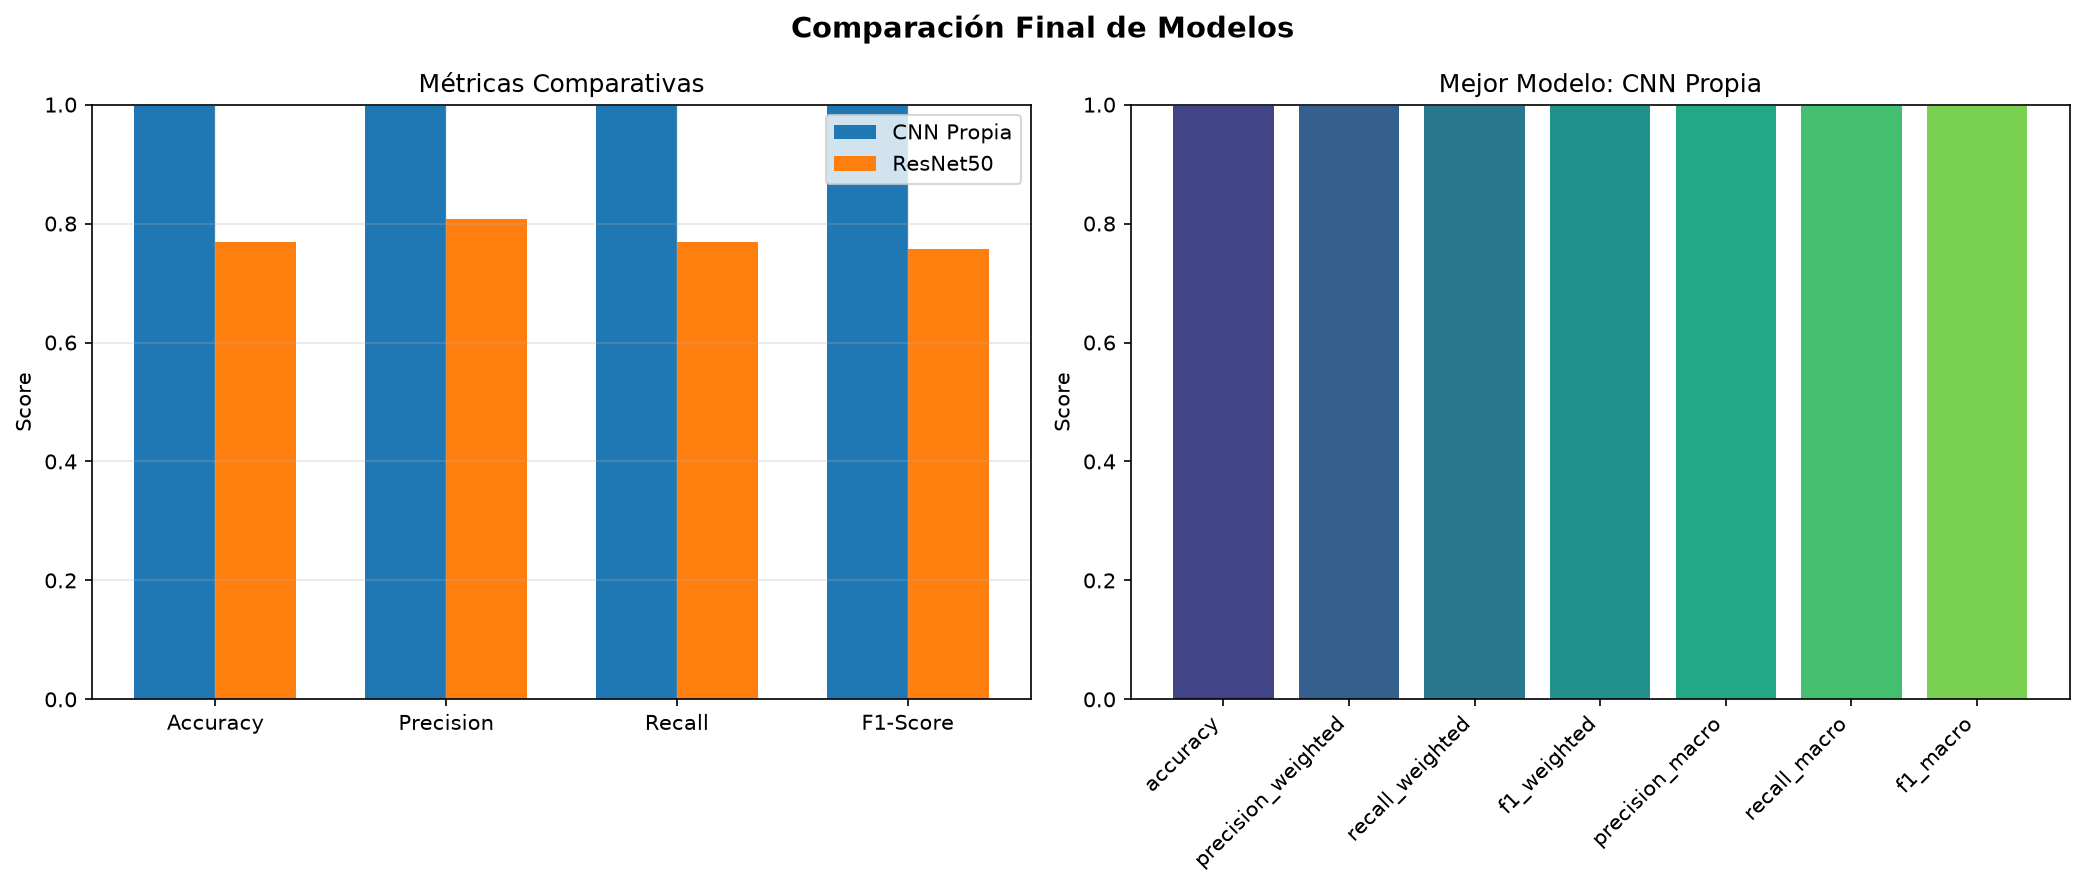
\includegraphics[width=0.62\textwidth]{images/final_comparison.png}
  \vspace{0.1cm}
  \footnotesize La CNN propia gana en las 4 métricas, y de forma pareja entre clases (el resultado \textit{macro} es igual de alto que el \textit{weighted}).
\end{frame}

\begin{frame}{Matrices de confusión}
  \centering
  \begin{columns}[T]
    \begin{column}{0.48\textwidth}
      \centering
      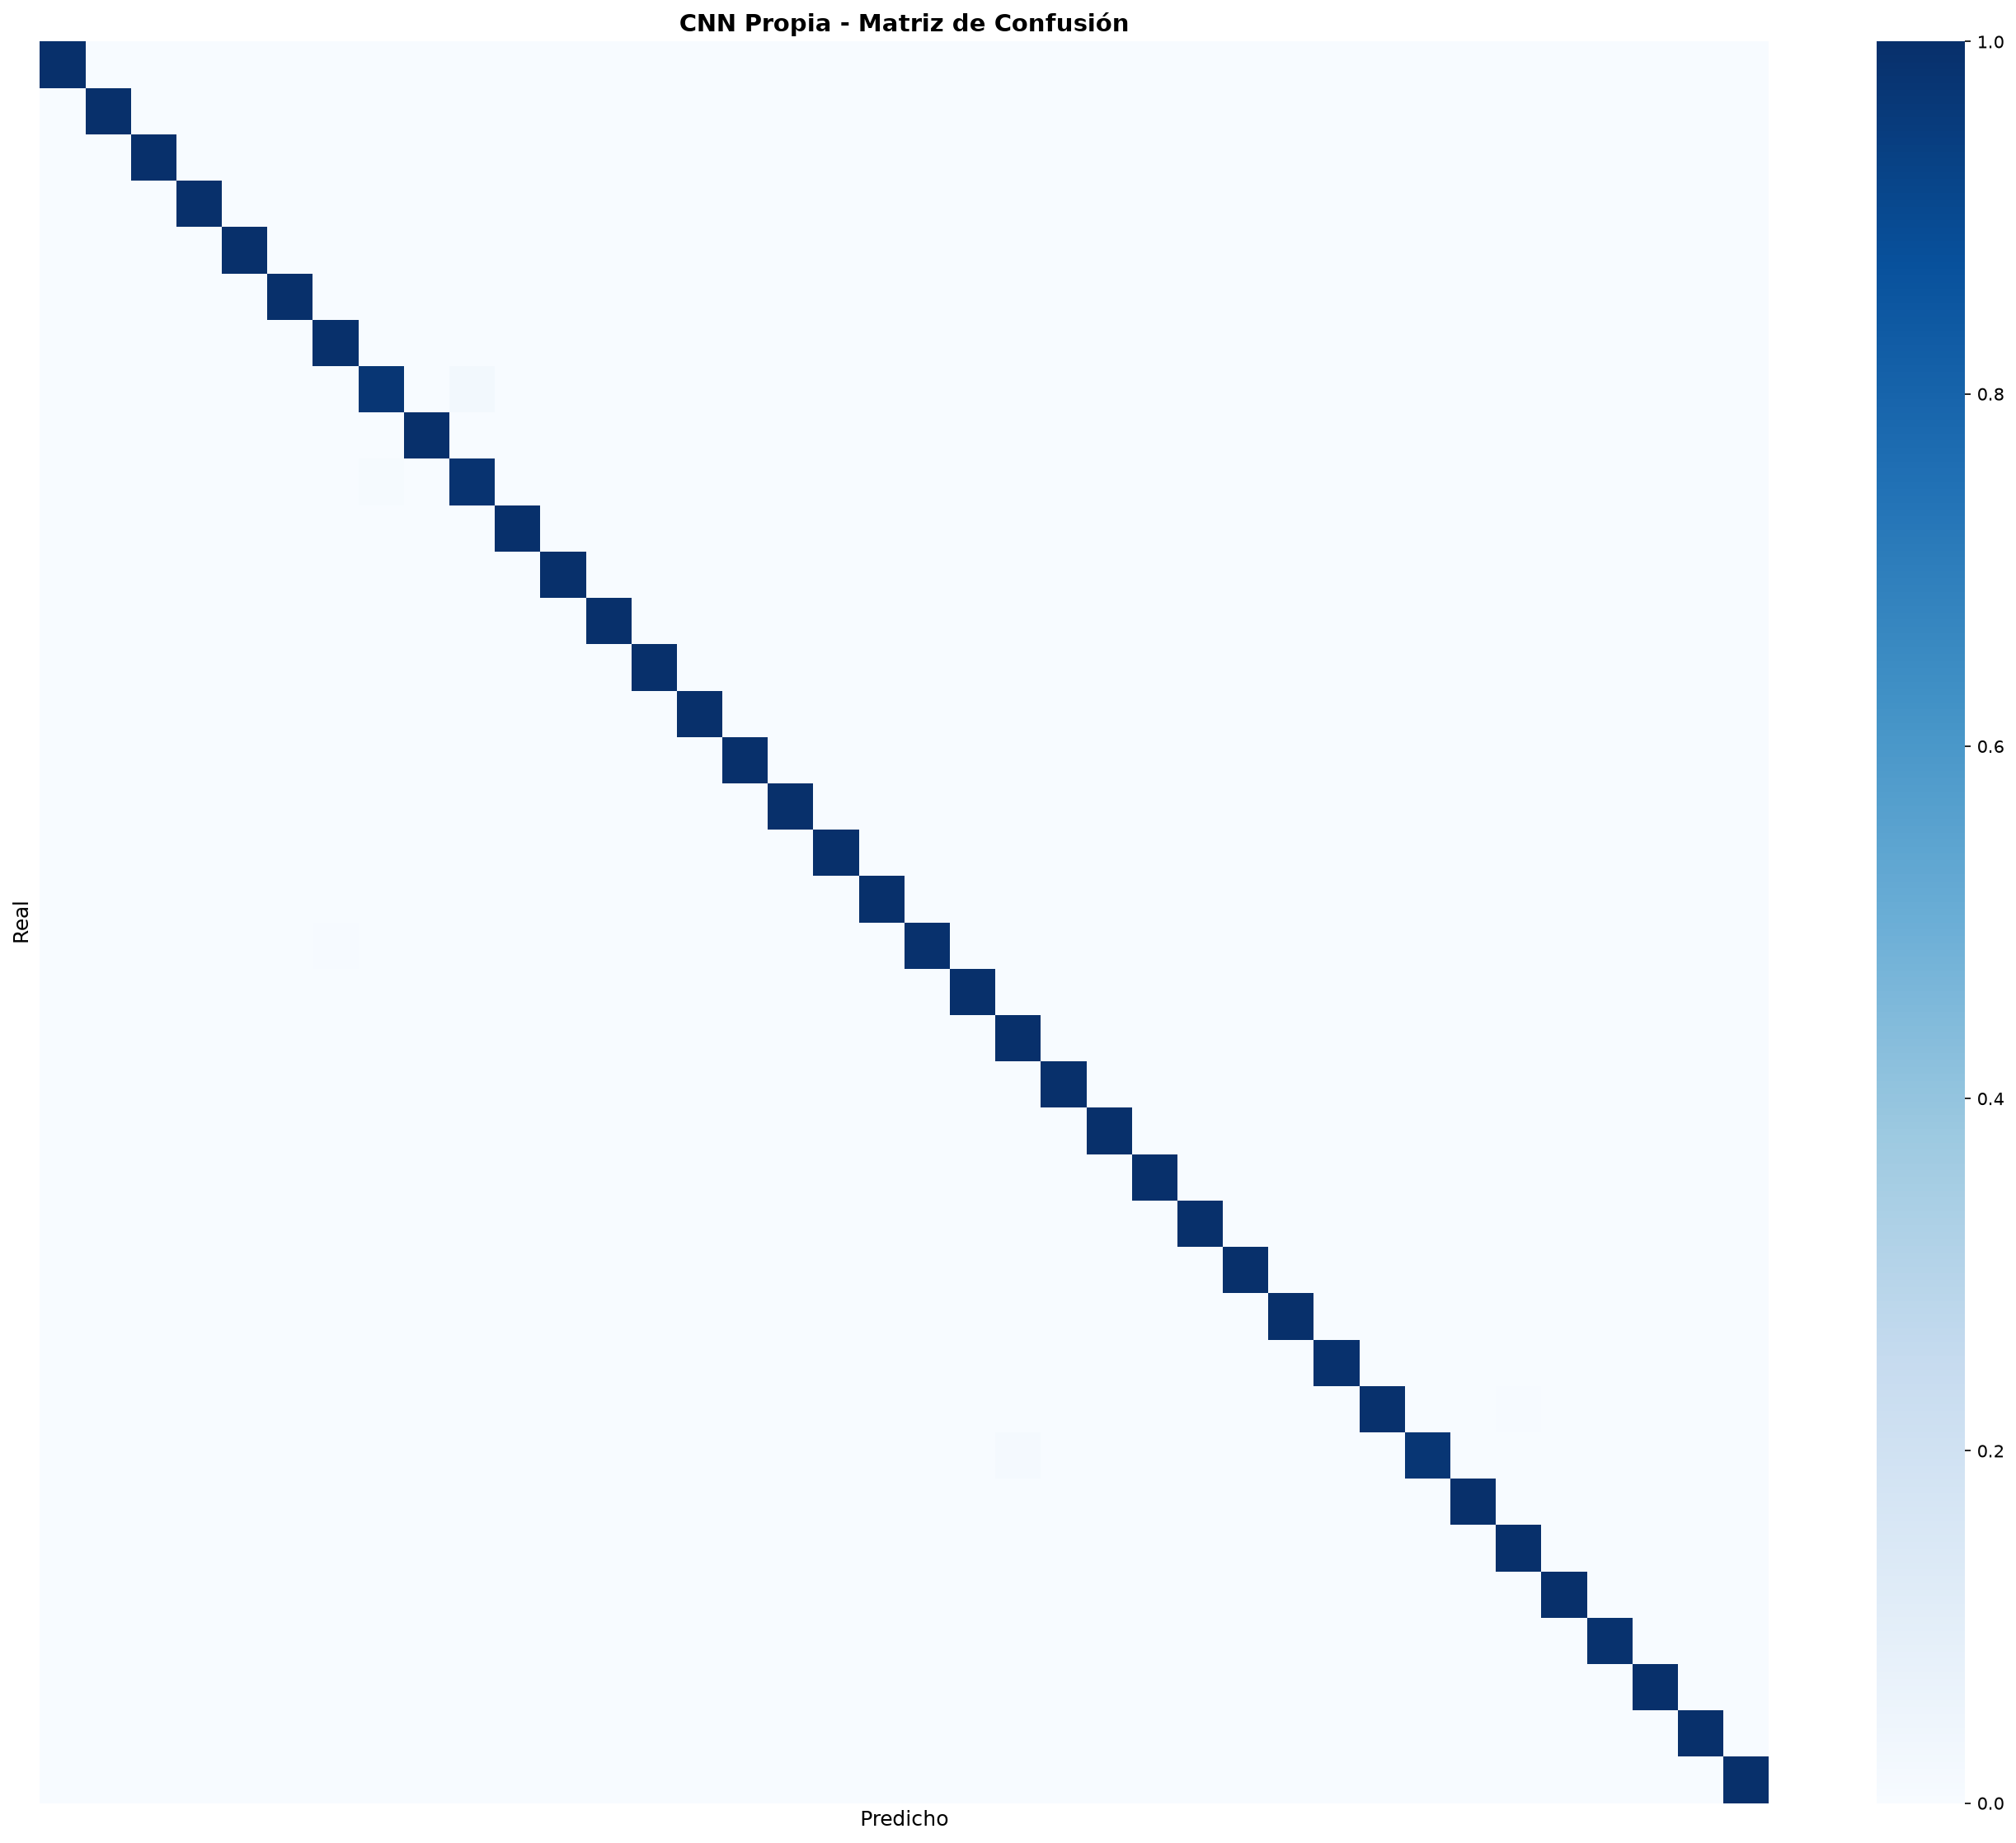
\includegraphics[width=\textwidth]{images/cnn_propia_confusion_matrix.png}\\
      \footnotesize CNN Propia
    \end{column}
    \begin{column}{0.48\textwidth}
      \centering
      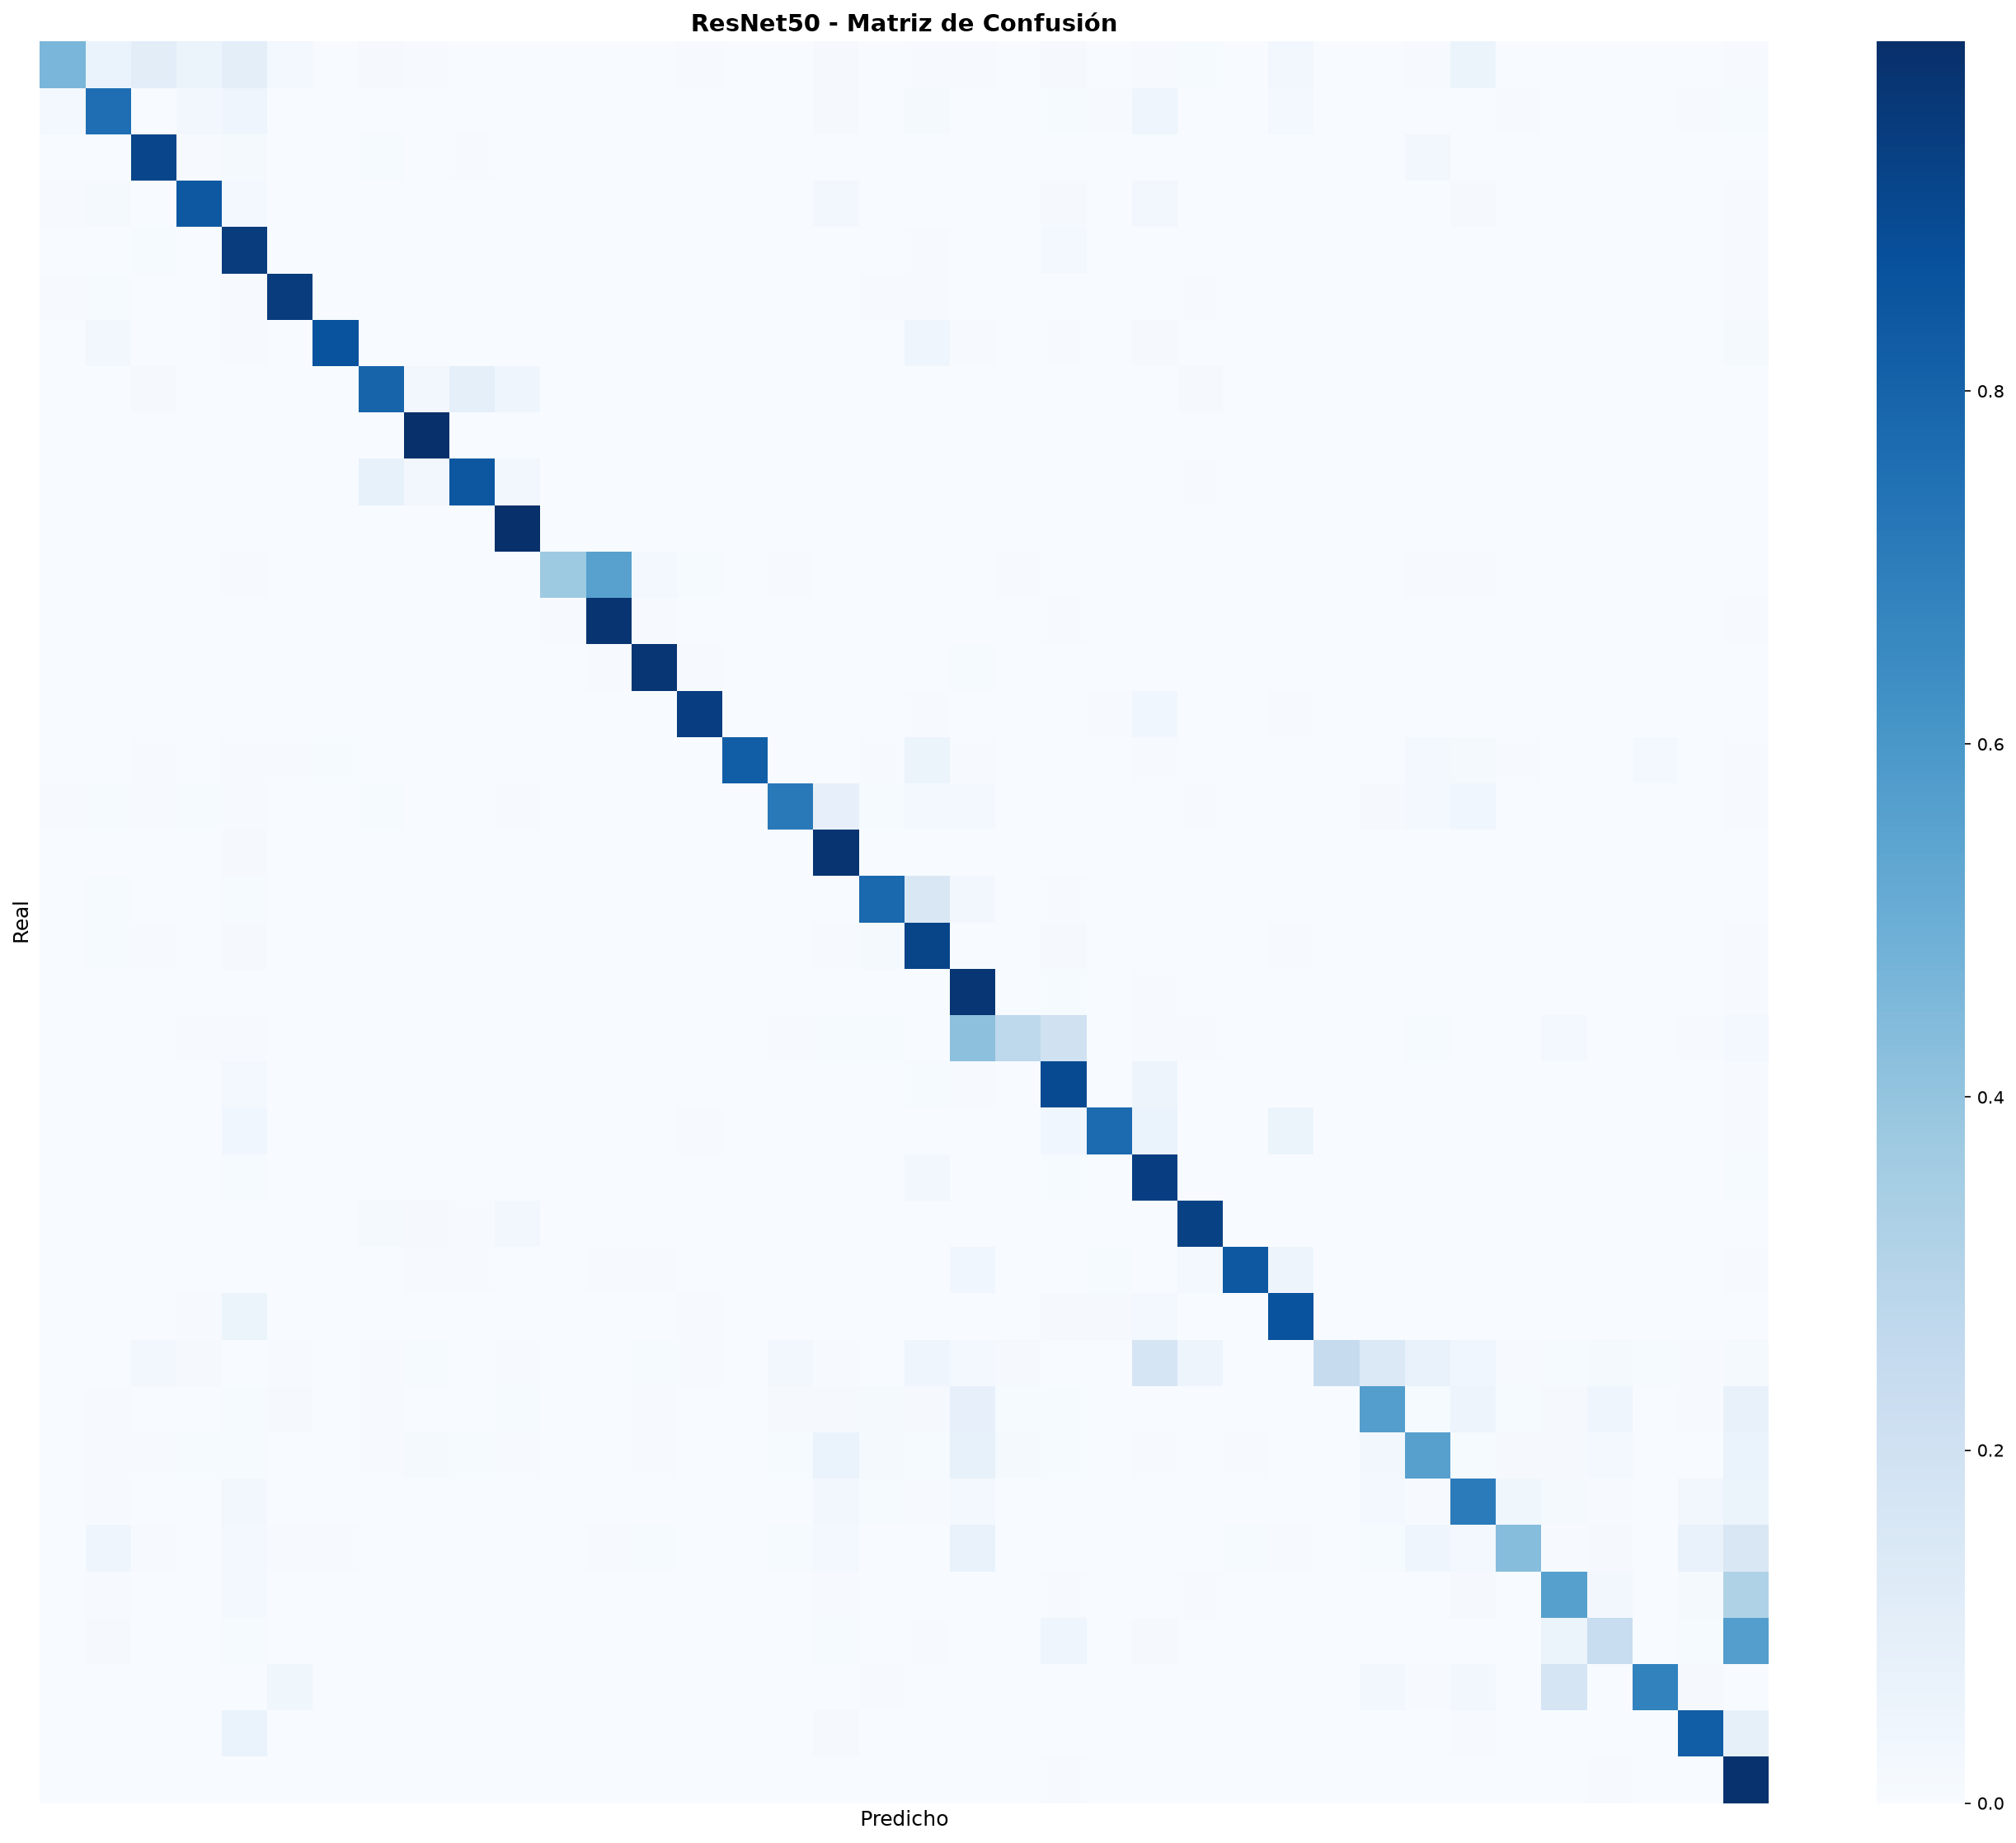
\includegraphics[width=\textwidth]{images/resnet50_confusion_matrix.png}\\
      \footnotesize ResNet50
    \end{column}
  \end{columns}
  \vspace{0.3cm}
  \footnotesize
  \begin{itemize}
    \item La diagonal de la CNN propia es prácticamente sólida (casi sin errores visibles).
    \item ResNet50 también acierta en la mayoría de los casos, pero confunde más clases vecinas — típicamente distintas enfermedades de un mismo cultivo.
  \end{itemize}
\end{frame}

% ===========================================================
\section{Rol 2 — Backend / DevOps Engineer}

\begin{frame}{Rol 2 — Responsabilidades}
  \begin{block}{Equivalente a: Backend + QA/DevOps}
  \end{block}
  \begin{itemize}
    \item Desarrolla la API con Flask, exponiendo el endpoint \texttt{/predict}.
    \item Empaqueta el modelo entrenado y la API para su despliegue en un servidor Linux.
    \item Despliega la API en consola (sin entorno gráfico), usando Docker.
    \item Configura logs, variables de entorno y reinicio automático del servicio.
  \end{itemize}
\end{frame}

\begin{frame}{Arquitectura de la API}
  \begin{itemize}
    \item \textbf{Flask} con tres endpoints:
    \begin{itemize}
      \item \texttt{POST /predict} — recibe una imagen, responde cultivo + enfermedad + probabilidad.
      \item \texttt{GET /health} — estado del servicio y si el modelo está cargado.
      \item \texttt{GET /model/info} — arquitectura y número de parámetros del modelo activo.
    \end{itemize}
  \end{itemize}
  \begin{block}{Ejemplo de respuesta — \texttt{POST /predict}}
    \texttt{\{"cultivo": "Tomate", "enfermedad": "Late blight", "probabilidad": 36.9\}}
  \end{block}
  \footnotesize El nombre de clase técnico del dataset (en inglés) se traduce a cultivo en español antes de responder, tal como exige la especificación del proyecto.
\end{frame}

\begin{frame}{Despliegue con Docker}
  \begin{itemize}
    \item Imagen basada en \texttt{python:3.11-slim}, con \texttt{gunicorn} sirviendo la API (2 workers).
    \item \texttt{HEALTHCHECK} integrado (\texttt{curl /health} cada 30s) para que Docker detecte si el servicio deja de responder.
    \item \texttt{.dockerignore} excluye dataset, entorno virtual y material que no necesita el contenedor (ej. la presentación).
  \end{itemize}
  \begin{alertblock}{Reto real encontrado y corregido}
    El contenedor fallaba al cargar el modelo por una incompatibilidad de versión de Keras: la imagen base solo permitía instalar una versión más antigua que la usada para guardar los modelos. Se corrigió actualizando la imagen base y fijando la versión exacta de Keras en \texttt{requirements.txt}.
  \end{alertblock}
\end{frame}

\begin{frame}{Verificación end-to-end}
  \begin{itemize}
    \item \texttt{docker build} + \texttt{docker run} — contenedor levantado y verificado como \textbf{healthy}.
    \item \texttt{GET /health} $\to$ \texttt{200 OK}, modelo cargado, 38 clases.
    \item \texttt{POST /predict} con imagen real $\to$ respuesta correcta en formato JSON.
    \item Frontend y archivos estáticos servidos correctamente desde el mismo contenedor (\texttt{GET /}, \texttt{/static/*}).
  \end{itemize}
  \begin{block}{Resultado}
    API completamente funcional dentro de Docker, sin depender de ningún proceso local.
  \end{block}
\end{frame}

% ===========================================================
\section{Rol 3 — Frontend Engineer / QA}

\begin{frame}{Rol 3 — Responsabilidades}
  \begin{block}{Equivalente a: Frontend + parte de QA}
  \end{block}
  \begin{itemize}
    \item Desarrolla la aplicación web (HTML/CSS/JS) para cargar una imagen.
    \item Consume el endpoint \texttt{/predict} y muestra el resultado al usuario de forma clara.
    \item Valida el formato de la respuesta JSON y maneja errores (imagen inválida, servidor caído, etc.).
    \item Realiza pruebas funcionales de extremo a extremo (QA) sobre el flujo completo.
  \end{itemize}
\end{frame}

\begin{frame}{Frontend — funcionalidades}
  \centering
  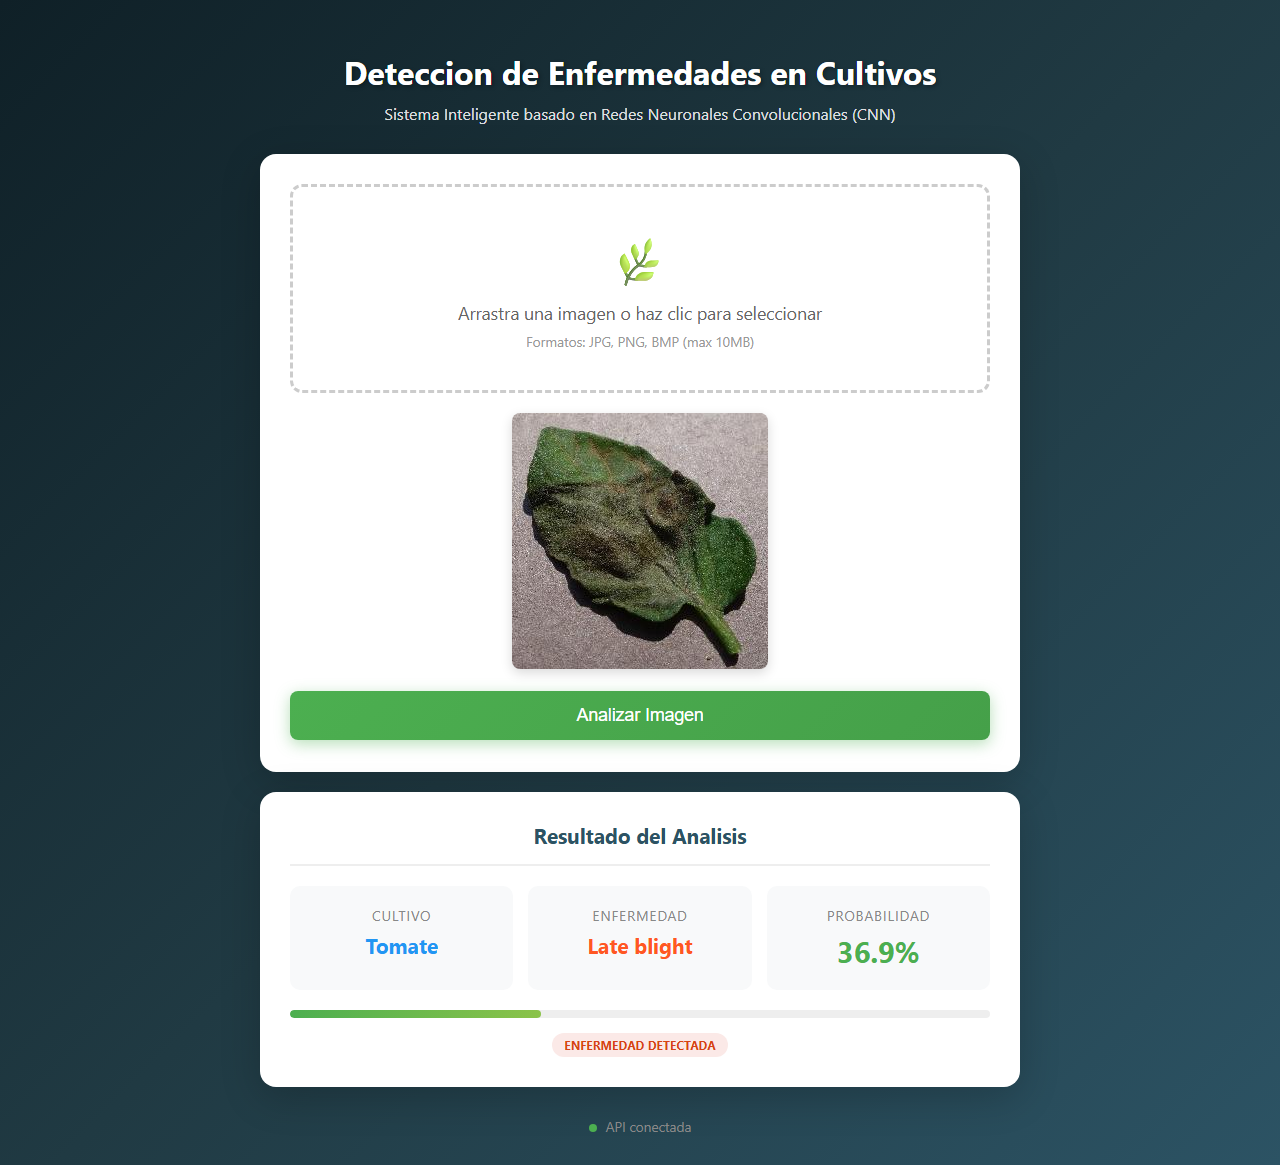
\includegraphics[width=0.42\textwidth]{images/frontend_resultado.png}
  \vspace{0.15cm}
  \footnotesize
  \begin{itemize}
    \item Selección de imagen por arrastrar-y-soltar o clic, con vista previa antes de analizar.
    \item Validación en el cliente: formato (JPG/PNG/BMP) y tamaño máximo (10\,MB).
    \item Indicador de conexión con la API en tiempo real (\textit{``API conectada''}, revisado cada 30s vía \texttt{/health}).
    \item Resultado mostrado con cultivo, enfermedad, probabilidad (barra animada) y una etiqueta de estado (sano / enfermedad detectada).
  \end{itemize}
\end{frame}

\begin{frame}{QA end-to-end: pruebas y hallazgos}
  \begin{itemize}
    \item Se probó el flujo completo (subir imagen $\to$ analizar $\to$ ver resultado) de forma automatizada con un navegador headless, además de pruebas manuales.
  \end{itemize}
  \begin{alertblock}{Bugs reales encontrados y corregidos}
    \begin{itemize}
      \item La API devolvía el cultivo en inglés (ej. \textit{``Apple''}) en vez de español (\textit{``Manzana''}), como exige la especificación — corregido con una tabla de traducción.
      \item Los archivos \texttt{CSS} y \texttt{JS} del frontend devolvían error 404 por un conflicto de rutas en Flask (una ruta automática interceptaba a la manual) — el frontend cargaba sin estilos ni interactividad. Corregido reconfigurando la carpeta estática de Flask.
    \end{itemize}
  \end{alertblock}
  \footnotesize Ambos bugs solo se detectaron probando el sistema de punta a punta, no revisando el código de forma aislada.
\end{frame}

% ===========================================================
\section{Cierre}

\begin{frame}{Estado final del proyecto}
  \centering
  \begin{tabular}{p{6cm}p{3.5cm}}
    \toprule
    \textbf{Fase} & \textbf{Estado} \\
    \midrule
    1-2. Exploración y Preprocesamiento & \textcolor{okgreen}{\textbf{Completada}} \\
    3. CNN propia & \textcolor{okgreen}{\textbf{Completada}} \\
    4. Transfer Learning (ResNet50) & \textcolor{okgreen}{\textbf{Completada}} \\
    5. Evaluación comparativa & \textcolor{okgreen}{\textbf{Completada}} \\
    6. API + Docker & \textcolor{okgreen}{\textbf{Completada}} \\
    7. Frontend & \textcolor{okgreen}{\textbf{Completada}} \\
    Subida a GitHub & \textcolor{okgreen}{\textbf{Completada}} \\
    \bottomrule
  \end{tabular}
\end{frame}

% ---------------------------------------------------------
\begin{frame}
  \centering
  \Large \textbf{¡Gracias!}\\[0.5cm]
  \normalsize Preguntas y comentarios
\end{frame}

\end{document}
